\section{Diagramma dei casi d'uso}\label{sec:casi-uso}
Il diagramma mostra le funzioni offerte ai tre ruoli di DriveHub. L'attore generale \emph{User} raccoglie registrazione e accesso; \emph{Customer}, \emph{Salesman} e \emph{Manager} ereditano queste possibilità e accedono alle operazioni delle rispettive aree. Il Customer consulta il catalogo e avvia le operazioni commerciali; il Salesman valuta le proposte e segue le pratiche; il Manager mantiene catalogo e sconti e consulta le vendite. I sei casi d'uso dettagliati sotto comprendono quattro operazioni del Customer, l'autorizzazione di un acquisto da parte del Salesman e la gestione di uno sconto da parte del Manager.

\begin{figure}[H]\centering
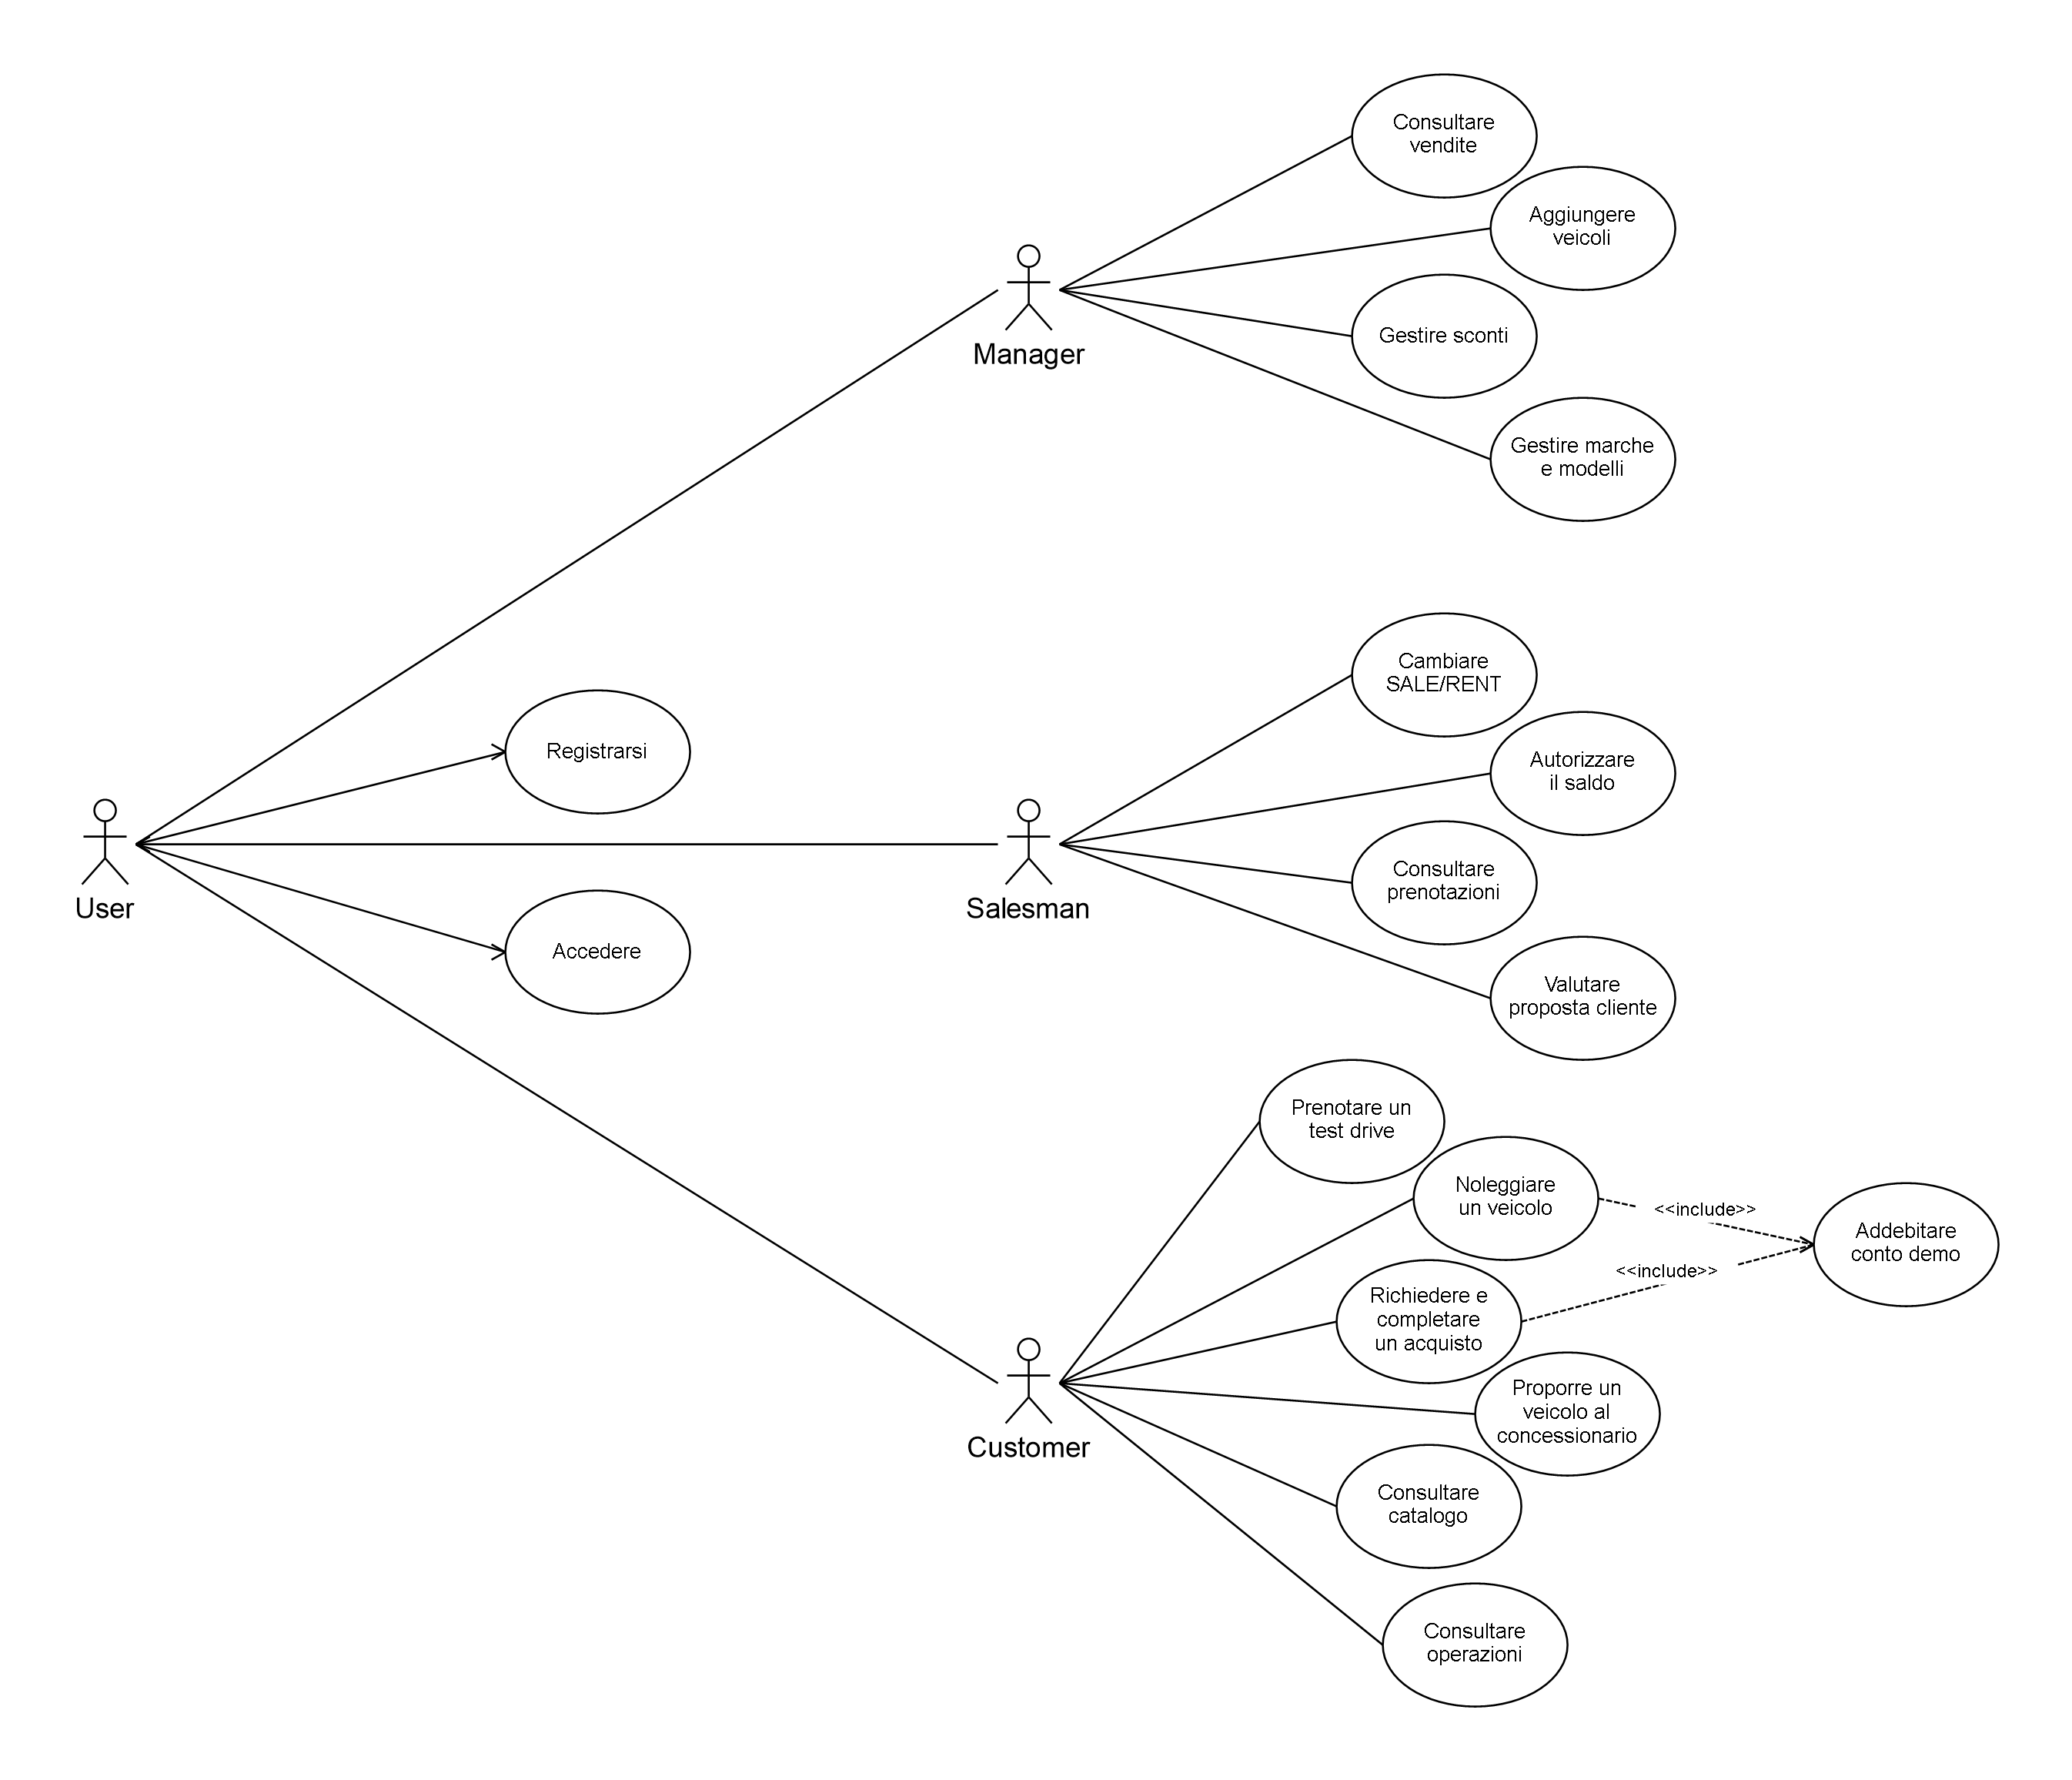
\includegraphics[width=\linewidth,height=.42\textheight,keepaspectratio]{users-swe-current.png}
\caption{Casi d'uso di DriveHub nel codice corrente. Diagramma sorgente: \texttt{docs/Users\ SWE.drawio}.}\label{fig:uc-correnti}
\end{figure}
\clearpage

\section{Template dei casi principali}
Ogni caso d'uso specifica nome, livello, descrizione, pre-condizioni, post-condizioni, attori, test e flussi. Il flusso principale è numerato a partire da 1 in ciascun template. Le alternative sono identificate da A1, A2 e così via, con il rimando al passo principale da cui si diramano. I riferimenti ai test distinguono i comportamenti coperti dalle alternative prive di una prova specifica. Le anomalie implementative sono richiamate separatamente dai flussi quando necessario.
\begingroup\renewcommand{\arraystretch}{1.4}
\subsection{Prenotare un test drive}\label{sec:uc-test-drive}
\begin{xltabular}{\textwidth}{| >{\bfseries}p{.22\textwidth} | >{\raggedright\arraybackslash}X |}
\caption{Caso d'uso: Prenotare un test drive}\label{tab:uc-test-drive}\\
\hline
\rowcolor{gray!15} Campo & \textbf{Contenuto}\\\hline
\endfirsthead
\multicolumn{2}{c}{{\tablename\ \thetable{} -- Continua dalla pagina precedente}}\\
\hline
\rowcolor{gray!15} Campo & \textbf{Contenuto}\\\hline
\endhead
\hline
\multicolumn{2}{r}{\textit{Continua nella pagina successiva...}}\\
\endfoot
\endlastfoot
Nome & Prenotare un test drive\\\hline
Livello & Obiettivo Utente\\\hline
Descrizione & Il Customer prenota una prova di guida di un'ora per un veicolo disponibile nel catalogo.\\\hline
Pre-condizioni & Il Customer ha effettuato l'accesso; il veicolo esiste ed è in stato \code{SALE} o \code{RENT}; la data e la fascia oraria scelte non sono passate.\\\hline
Post-condizioni & Una prenotazione di test drive è registrata per il Customer, il veicolo e lo slot selezionato.\\\hline
Attori & Customer\\\hline
Test & \code{UserGoalsFunctionalTest.bookTestDrive} esercita il percorso principale su H2; \code{RentalWorkflowTest} verifica le regole dell'entità. Non è presente una prova funzionale specifica per ciascuna alternativa o per richieste concorrenti.\\\hline
Flusso Principale &
\begin{enumerate}[label=\arabic*.,start=1,leftmargin=*,nosep]
  \item Il Customer seleziona un veicolo dal catalogo e apre la scheda dei test drive.
  \item Sceglie una data e uno degli orari proposti, dalle 09:00 alle 16:00.
  \item Il sistema verifica che il veicolo sia idoneo, che il Customer abbia meno di tre test drive futuri e che il veicolo non sia noleggiato nella data scelta.
  \item Il sistema verifica che lo slot di un'ora non sia già occupato per quel veicolo.
  \item Il sistema salva la prenotazione e ne comunica l'esito al Customer.
\end{enumerate}\\\hline
Flussi Alternativi &
\textbf{A1 (passo 2). Data o orario non validi:} se lo slot è nel passato o fuori dalla fascia consentita, il sistema rifiuta la prenotazione.\newline\newline
\textbf{A2 (passo 3). Veicolo non idoneo o limite raggiunto:} un veicolo non in vendita né a noleggio, oppure tre test drive futuri già registrati, impedisce il salvataggio.\newline\newline
\textbf{A3 (passi 3--4). Veicolo indisponibile:} un noleggio nel giorno scelto o un altro test drive nello stesso slot produce un conflitto.\newline\newline
\textbf{A4 (passo 4). Richieste concorrenti:} il controllo dello slot precede l'inserimento; il database non impone un vincolo univoco sullo slot, quindi due richieste simultanee potrebbero entrambe riuscire. Inoltre il servizio riconduce i minuti forniti all'inizio dell'ora: un input diretto come 10:30 è trattato come 10:00.\\\hline
\end{xltabular}

\endgroup
\begingroup\renewcommand{\arraystretch}{1.4}
\subsection{Noleggiare un veicolo}\label{sec:uc-noleggio}
\begin{xltabular}{\textwidth}{| >{\bfseries}p{.22\textwidth} | >{\raggedright\arraybackslash}X |}
\caption{Caso d'uso: Noleggiare un veicolo}\label{tab:uc-noleggio}\\
\hline
\rowcolor{gray!15} Campo & \textbf{Contenuto}\\\hline
\endfirsthead
\multicolumn{2}{c}{{\tablename\ \thetable{} -- Continua dalla pagina precedente}}\\
\hline
\rowcolor{gray!15} Campo & \textbf{Contenuto}\\\hline
\endhead
\hline
\multicolumn{2}{r}{\textit{Continua nella pagina successiva...}}\\
\endfoot
\endlastfoot
Nome & Noleggiare un veicolo\\\hline
Livello & Obiettivo Utente\\\hline
Descrizione & Il Customer prenota un veicolo per un intervallo di giorni e paga anticipatamente l'intero importo con il conto dimostrativo.\\\hline
Pre-condizioni & Il Customer ha effettuato l'accesso; il veicolo esiste ed è in stato \code{RENT}; la data iniziale non è passata e la data finale non precede quella iniziale.\\\hline
Post-condizioni & Il noleggio è registrato, l'importo è sottratto dal saldo del Customer e i test drive sul veicolo nei giorni prenotati sono cancellati. Le scritture nel database avvengono nella stessa transazione.\\\hline
Attori & Customer\\\hline
Test & \code{RentalServiceTest.bookRentalDebitsAccount} verifica il servizio con DAO simulati; \code{CheckoutFunctionalTest.rentalBookingWorkflow} verifica il percorso principale su H2. Le alternative di conflitto e la concorrenza non hanno un test funzionale dedicato nella suite corrente.\\\hline
Flusso Principale &
\begin{enumerate}[label=\arabic*.,start=1,leftmargin=*,nosep]
  \item Il Customer seleziona un veicolo disponibile per il noleggio e indica il primo e l'ultimo giorno.
  \item Il sistema mostra un preventivo. Nel conteggio sono inclusi sia il giorno iniziale sia quello finale.
  \item Il Customer conferma la prenotazione.
  \item Il sistema verifica che non vi siano noleggi sovrapposti e calcola l'importo: tariffa giornaliera pari allo 0,1\% del prezzo del veicolo, con un fattore 0,95 applicato per ogni giorno aggiuntivo.
  \item Il sistema addebita l'intero importo sul conto dimostrativo e registra il noleggio.
  \item Il sistema cancella gli eventuali test drive sul veicolo nei giorni prenotati e conferma l'operazione.
\end{enumerate}\\\hline
Flussi Alternativi &
\textbf{A1 (passo 1). Veicolo o date non validi:} il sistema rifiuta la richiesta senza registrare il noleggio.\newline\newline
\textbf{A2 (passo 4). Periodo occupato:} se esiste un noleggio che condivide almeno un giorno, l'operazione è rifiutata.\newline\newline
\textbf{A3 (passo 4). Richieste concorrenti:} la verifica delle sovrapposizioni non è protetta da un vincolo di esclusione nel database; due richieste simultanee potrebbero entrambe riuscire.\newline\newline
\textbf{A4 (passo 5). Saldo insufficiente:} l'addebito fallisce; la transazione annulla anche le altre scritture.\\\hline
\end{xltabular}

\endgroup
\clearpage
\begingroup\renewcommand{\arraystretch}{1.4}
\subsection{Richiedere e completare un acquisto}\label{sec:uc-acquisto}
\begin{xltabular}{\textwidth}{| >{\bfseries}p{.22\textwidth} | >{\raggedright\arraybackslash}X |}
\caption{Caso d'uso: Richiedere e completare un acquisto}\label{tab:uc-acquisto}\\
\hline
\rowcolor{gray!15} Campo & \textbf{Contenuto}\\\hline
\endfirsthead
\multicolumn{2}{c}{{\tablename\ \thetable{} -- Continua dalla pagina precedente}}\\
\hline
\rowcolor{gray!15} Campo & \textbf{Contenuto}\\\hline
\endhead
\hline
\multicolumn{2}{r}{\textit{Continua nella pagina successiva...}}\\
\endfoot
\endlastfoot
Nome & Richiedere e completare un acquisto\\\hline
Livello & Obiettivo Utente\\\hline
Descrizione & Il Customer riserva un veicolo in vendita versando un acconto; dopo l'autorizzazione del Salesman, paga il saldo e conclude l'acquisto. Le azioni possono avvenire in sessioni diverse.\\\hline
Pre-condizioni & Customer e Salesman hanno effettuato l'accesso alle rispettive aree; il veicolo esiste ed è in stato \code{SALE}; il Customer dispone dell'importo necessario per l'acconto.\\\hline
Post-condizioni & Dopo l'acconto il veicolo è \code{BLOCKED} e la richiesta è registrata. Dopo il saldo il veicolo è \code{SOLD}, la richiesta è eliminata, la vendita è registrata e gli eventuali test drive futuri sono cancellati. Ciascuna fase ha una propria transazione.\\\hline
Attori & Customer (primario), Salesman\\\hline
Schermate & Passi 1--2: catalogo (figura~\ref{fig:ui-catalogo}); passo 3: richieste Salesman (figura~\ref{fig:ui-salesman-richieste}); passi 4--6: acquisti del Customer (figura~\ref{fig:ui-acquisti}) e conto (figura~\ref{fig:ui-conto}).\\\hline
Test & \code{CheckoutFunctionalTest.completePurchaseWorkflow} verifica il percorso principale su H2; \code{cancelPurchaseWorkflowWithPenalty} verifica l'annullamento. \code{SalesServiceTest} verifica avvio e penale con mock. Autorizzazione assente, scadenza e variazione del prezzo non sono coperti da una prova funzionale dedicata.\\\hline
Flusso Principale &
\begin{enumerate}[leftmargin=*,nosep]
  \item Il Customer seleziona un veicolo in vendita; l'interfaccia calcola l'acconto, pari al 20\% del prezzo visualizzato. Il saldo finale usa invece \code{Vehicle.price}, che può differire dal prezzo visualizzato in presenza di sconti.
  \item Il Customer conferma: il sistema addebita l'acconto, registra la richiesta e blocca il veicolo.
  \item Il Salesman consulta la richiesta e la autorizza; il sistema registra il venditore e fissa la scadenza a un mese.
  \item Il Customer seleziona la richiesta autorizzata e conferma il pagamento del saldo.
  \item Il sistema calcola la differenza tra il prezzo corrente del veicolo e l'acconto già versato, quindi addebita l'eventuale residuo.
  \item Il sistema registra la vendita, elimina la richiesta, pone il veicolo in stato \code{SOLD} e cancella i test drive futuri relativi al veicolo.
\end{enumerate}\\\hline
Flussi Alternativi &
\textbf{2. Veicolo non disponibile o saldo insufficiente:} la richiesta non viene creata e le scritture della fase sono annullate.\newline\newline
\textbf{4. Autorizzazione assente:} l'interfaccia impedisce di avviare il saldo. Il servizio di completamento non verifica autonomamente autorizzazione e scadenza: una chiamata diretta potrebbe aggirare quel controllo.\newline\newline
\textbf{4. Annullamento o scadenza:} la richiesta viene eliminata e il veicolo torna in vendita; il sistema trattiene il 20\% dell'acconto e rimborsa l'80\%. Le richieste scadute sono elaborate all'avvio e durante alcune consultazioni, senza un timer dedicato.\newline\newline
\textbf{5. Prezzo variato:} la richiesta non conserva un prezzo finale bloccato; il residuo è calcolato sul prezzo del veicolo letto al momento del saldo.\\\hline
\end{xltabular}

\endgroup
\begingroup\renewcommand{\arraystretch}{1.4}
\subsection{Proporre un veicolo al concessionario}\label{sec:uc-cessione}
\begin{xltabular}{\textwidth}{| >{\bfseries}p{.22\textwidth} | >{\raggedright\arraybackslash}X |}
\caption{Caso d'uso: Proporre un veicolo al concessionario}\label{tab:uc-cessione}\\
\hline
\rowcolor{gray!15} Campo & \textbf{Contenuto}\\\hline
\endfirsthead
\multicolumn{2}{c}{{\tablename\ \thetable{} -- Continua dalla pagina precedente}}\\
\hline
\rowcolor{gray!15} Campo & \textbf{Contenuto}\\\hline
\endhead
\hline
\multicolumn{2}{r}{\textit{Continua nella pagina successiva...}}\\
\endfoot
\endlastfoot
Nome & Proporre un veicolo al concessionario\\\hline
Livello & Obiettivo Utente\\\hline
Descrizione & Il Customer propone alla concessionaria il proprio veicolo. Il sistema calcola una valutazione; un Salesman può accettare la proposta e accreditare l'importo sul conto dimostrativo del Customer.\\\hline
Pre-condizioni & Il Customer ha effettuato l'accesso; sceglie marca e modello, inserisce VIN, chilometri e anno di immatricolazione validi. Se manca la targa, i chilometri devono essere zero.\\\hline
Post-condizioni & Dopo l'invio, il veicolo è in stato \code{WAITING} e la proposta è registrata. Se accettata, l'importo è accreditato al Customer, la proposta è eliminata, la spesa della concessionaria è registrata e il veicolo passa a \code{SALE}. Invio e decisione sono due transazioni distinte.\\\hline
Attori & Customer (primario), Salesman\\\hline
Test & \code{CheckoutFunctionalTest.customerProposeAndApprove} esercita proposta e approvazione su H2. Rifiuto, riuso di VIN \code{SOLD} e accredito fallito non hanno un test funzionale dedicato nella suite corrente.\\\hline
Flusso Principale &
\begin{enumerate}[label=\arabic*.,start=1,leftmargin=*,nosep]
  \item Il Customer apre la schermata di vendita del proprio veicolo e seleziona marca e modello.
  \item Inserisce VIN, eventuale targa, chilometri e anno di immatricolazione.
  \item Il sistema mostra una valutazione calcolata dal prezzo di listino del modello, tenendo conto di targa, età e chilometri.
  \item Il Customer conferma la proposta; il sistema registra il veicolo in stato \code{WAITING} e la richiesta con l'importo stimato.
  \item Il Salesman esamina i veicoli in attesa e approva la proposta.
  \item Il sistema accredita la valutazione al Customer, registra l'operazione con importo negativo per la concessionaria, elimina la richiesta e mette il veicolo in vendita.
\end{enumerate}\\\hline
Flussi Alternativi &
\textbf{A1 (passo 2). Dati non validi:} l'interfaccia rifiuta VIN mancante o troppo lungo, chilometri negativi, anno fuori intervallo e veicolo senza targa con chilometri diversi da zero.\newline\newline
\textbf{A2 (passo 4). VIN già attivo:} se il VIN appartiene a un veicolo non \code{SOLD}, la proposta è rifiutata. Se il VIN appartiene a un veicolo \code{SOLD}, il sistema riutilizza quella scheda e la pone in stato \code{WAITING}.\newline\newline
\textbf{A3 (passo 5). Proposta rifiutata:} il Salesman elimina la richiesta; il veicolo torna \code{SOLD} se ha operazioni precedenti, altrimenti viene eliminato dal catalogo.\newline\newline
\textbf{A4 (passo 6). Accredito non riuscito:} le modifiche della decisione vengono annullate dalla transazione.\\\hline
\end{xltabular}

\endgroup
\clearpage
\begingroup\renewcommand{\arraystretch}{1.4}
\subsection{Autorizzare una richiesta di acquisto}\label{sec:uc-autorizzazione}
\begin{xltabular}{\textwidth}{| >{\bfseries}p{.22\textwidth} | >{\raggedright\arraybackslash}X |}
\caption{Caso d'uso: Autorizzare una richiesta di acquisto}\label{tab:uc-autorizzazione}\\
\hline
\rowcolor{gray!15} Campo & \textbf{Contenuto}\\\hline
\endfirsthead
\multicolumn{2}{c}{{\tablename\ \thetable{} -- Continua dalla pagina precedente}}\\
\hline
\rowcolor{gray!15} Campo & \textbf{Contenuto}\\\hline
\endhead
\hline
\multicolumn{2}{r}{\textit{Continua nella pagina successiva...}}\\
\endfoot
\endlastfoot
Nome & Autorizzare una richiesta di acquisto\\\hline
Livello & Obiettivo Utente\\\hline
Descrizione & Il Salesman autorizza il Customer a completare un acquisto per cui è già stato versato un acconto. L'autorizzazione assegna il venditore alla pratica e stabilisce il termine per il saldo.\\\hline
Pre-condizioni & Il Salesman ha effettuato l'accesso alla propria area; esiste una richiesta di acquisto con acconto positivo e il relativo veicolo è stato riservato dal Customer.\\\hline
Post-condizioni & La richiesta conserva l'identificativo del Salesman e una scadenza pari alla data di autorizzazione più un mese. Il veicolo resta \code{BLOCKED}; in questa fase non avvengono addebiti.\\\hline
Attori & Salesman (primario), Customer (beneficiario dell'autorizzazione)\\\hline
Test & \code{CheckoutFunctionalTest.completePurchaseWorkflow} verifica che l'autorizzazione imposti la scadenza a un mese e che il successivo acquisto registri il venditore. La selezione nella GUI e i rami di errore non sono verificati da quel test.\\\hline
Flusso Principale &
\begin{enumerate}[label=\arabic*.,start=1,leftmargin=*,nosep]
  \item Il Salesman consulta le richieste di acquisto e seleziona la pratica da autorizzare.
  \item Attiva il comando di autorizzazione.
  \item Il sistema recupera la richiesta e verifica che si tratti di un acquisto, riconoscibile dall'acconto positivo.
  \item Il sistema salva nella richiesta l'identificativo del Salesman e la data di scadenza, in un'unica transazione.
  \item L'interfaccia conferma l'esito e aggiorna l'elenco. Il Customer può procedere al saldo dalla propria area.
\end{enumerate}\\\hline
Flussi Alternativi &
\textbf{A1 (passo 1). Nessuna richiesta selezionata:} l'interfaccia mostra un messaggio e non invia l'autorizzazione.\newline\newline
\textbf{A2 (passo 3). Richiesta assente o di tipo diverso:} una richiesta non più presente produce un errore; una proposta di cessione è rifiutata dall'interfaccia e dal servizio di autorizzazione. Nessuna autorizzazione viene salvata.\newline\newline
\textbf{A3 (passo 4). Salvataggio non riuscito:} la transazione viene annullata e l'interfaccia comunica l'errore.\\\hline
\end{xltabular}

\endgroup
\begingroup\renewcommand{\arraystretch}{1.4}
\subsection{Gestire lo sconto su un veicolo}\label{sec:uc-sconto}
\begin{xltabular}{\textwidth}{| >{\bfseries}p{.22\textwidth} | >{\raggedright\arraybackslash}X |}
\caption{Caso d'uso: Gestire lo sconto su un veicolo}\label{tab:uc-sconto}\\
\hline
\rowcolor{gray!15} Campo & \textbf{Contenuto}\\\hline
\endfirsthead
\multicolumn{2}{c}{{\tablename\ \thetable{} -- Continua dalla pagina precedente}}\\
\hline
\rowcolor{gray!15} Campo & \textbf{Contenuto}\\\hline
\endhead
\hline
\multicolumn{2}{r}{\textit{Continua nella pagina successiva...}}\\
\endfoot
\endlastfoot
Nome & Gestire lo sconto su un veicolo\\\hline
Livello & Obiettivo Utente\\\hline
Descrizione & Il Manager applica, modifica o rimuove una promozione sul singolo veicolo. Il catalogo del Customer considera questa percentuale nel calcolo del prezzo esposto.\\\hline
Pre-condizioni & Il Manager ha effettuato l'accesso alla propria area e il veicolo è presente nel catalogo.\\\hline
Post-condizioni & La percentuale di sconto del veicolo è salvata nel database. Il successivo calcolo del preventivo considera il maggiore fra sconto del veicolo e sconto del modello, senza sommarli.\\\hline
Attori & Manager\\\hline
Test & \code{UserGoalsFunctionalTest.managerVehicleDiscount} applica il 10\%, verifica la riduzione del preventivo e controlla il ritorno al prezzo precedente dopo la rimozione. Il test attraversa servizio e persistenza H2; non esercita i comandi della GUI né il saldo dell'acquisto.\\\hline
Flusso Principale &
\begin{enumerate}[label=\arabic*.,start=1,leftmargin=*,nosep]
  \item Il Manager consulta il parco veicoli e seleziona un esemplare.
  \item Inserisce una percentuale intera compresa fra 0 e 50 e attiva il comando per applicarla.
  \item Il sistema valida la percentuale e salva lo sconto del veicolo, sostituendo quello eventualmente già presente nella stessa transazione.
  \item L'interfaccia conferma l'esito e aggiorna i dati. Alla successiva consultazione del catalogo, il preventivo viene ricalcolato considerando la promozione salvata.
\end{enumerate}\\\hline
Flussi Alternativi &
\textbf{A1 (passo 1). Nessun veicolo selezionato:} l'interfaccia richiede una selezione e non invia modifiche.\newline\newline
\textbf{A2 (passo 2). Percentuale non valida:} campo vuoto, valore non intero o fuori dall'intervallo 0--50 causano un errore; lo sconto precedente resta invariato.\newline\newline
\textbf{A3 (passo 2). Rimozione dello sconto:} il Manager sceglie il comando di rimozione; il sistema elimina la promozione individuale. L'eventuale sconto del modello resta applicabile al preventivo.\newline\newline
\textbf{A4 (passo 3). Salvataggio non riuscito:} la transazione viene annullata e l'interfaccia comunica l'errore.\\\hline
\end{xltabular}
\noindent\textbf{Limite del flusso di acquisto.} Lo sconto interviene sul preventivo di catalogo; il saldo usa invece il prezzo memorizzato nel veicolo, secondo l'anomalia descritta nella sezione~\ref{sec:pricing}.

\endgroup
